\documentclass{exam}
\usepackage{../../mypackages}
\usepackage{../../macros}


\SolutionEmphasis{\color{blue}}
\renewcommand{\solutiontitle}{\noindent}


\title{Interrogation N°3 - Forces et diagrammes objet interaction}
\author{N. Bancel}
\date{5 Février 2025}

\begin{document}

\textbf{Collège Lycée Suger}
\hfill
\textbf{Physique-Chimie} \\

\textbf{Année 2024-2025 - 2ème trimestre}
\hfill
\textbf{3ème CI} \par

{\let\newpage\relax\maketitle}

\begin{center}
\textbf{\textcolor{red}{Durée : 45 minutes. Coefficient 2. La calculatrice n'est pas autorisée}} \\
\textbf{\textcolor{red}{Une réponse donnée sans justification sera considérée comme fausse.}} \\
Cette interrogation contient \numquestions\ questions, sur \numpages\ pages et est notée sur 20 points. 

\end{center}

\section*{Exercice 1 : Cours (4 points)}

\vspace{1em}

\begin{questions}
  \question[2] Quelles sont les 4 caractéristiques d'une force ?
  \question[2] Enoncer le principe d'inertie.
\end{questions}

\section*{Exercice 2 : Diagramme objet interaction (6 points)}
\begin{questions}
  \question[3] Un joueur de foot frappe une balle posée sur le sol. Réaliser le diagramme objet-interaction du ballon lorsque le joueur frappe la balle. 
  \begin{figure}[H]
    \centering
    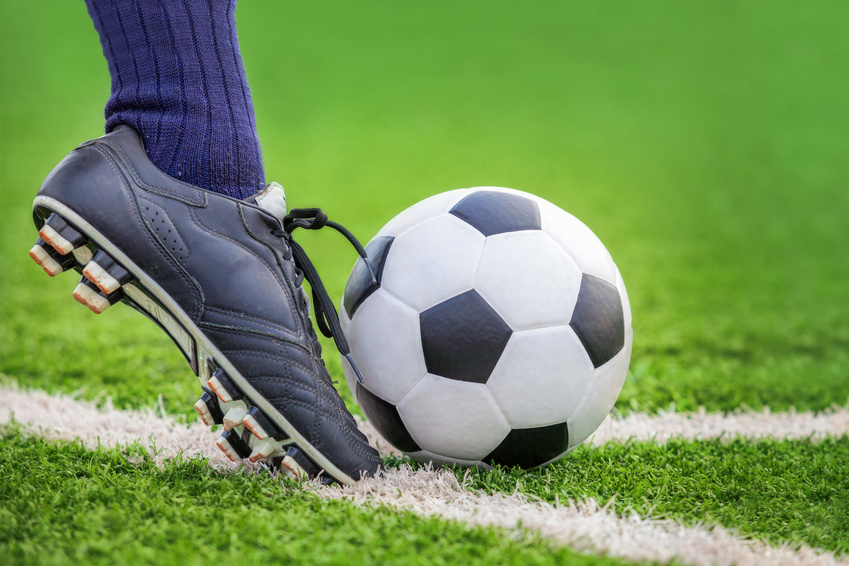
\includegraphics[width=0.4\linewidth]{img/interro_03_03.jpg}
  \end{figure}
  \begin{solution}
    \begin{figure}[H]
      \centering
      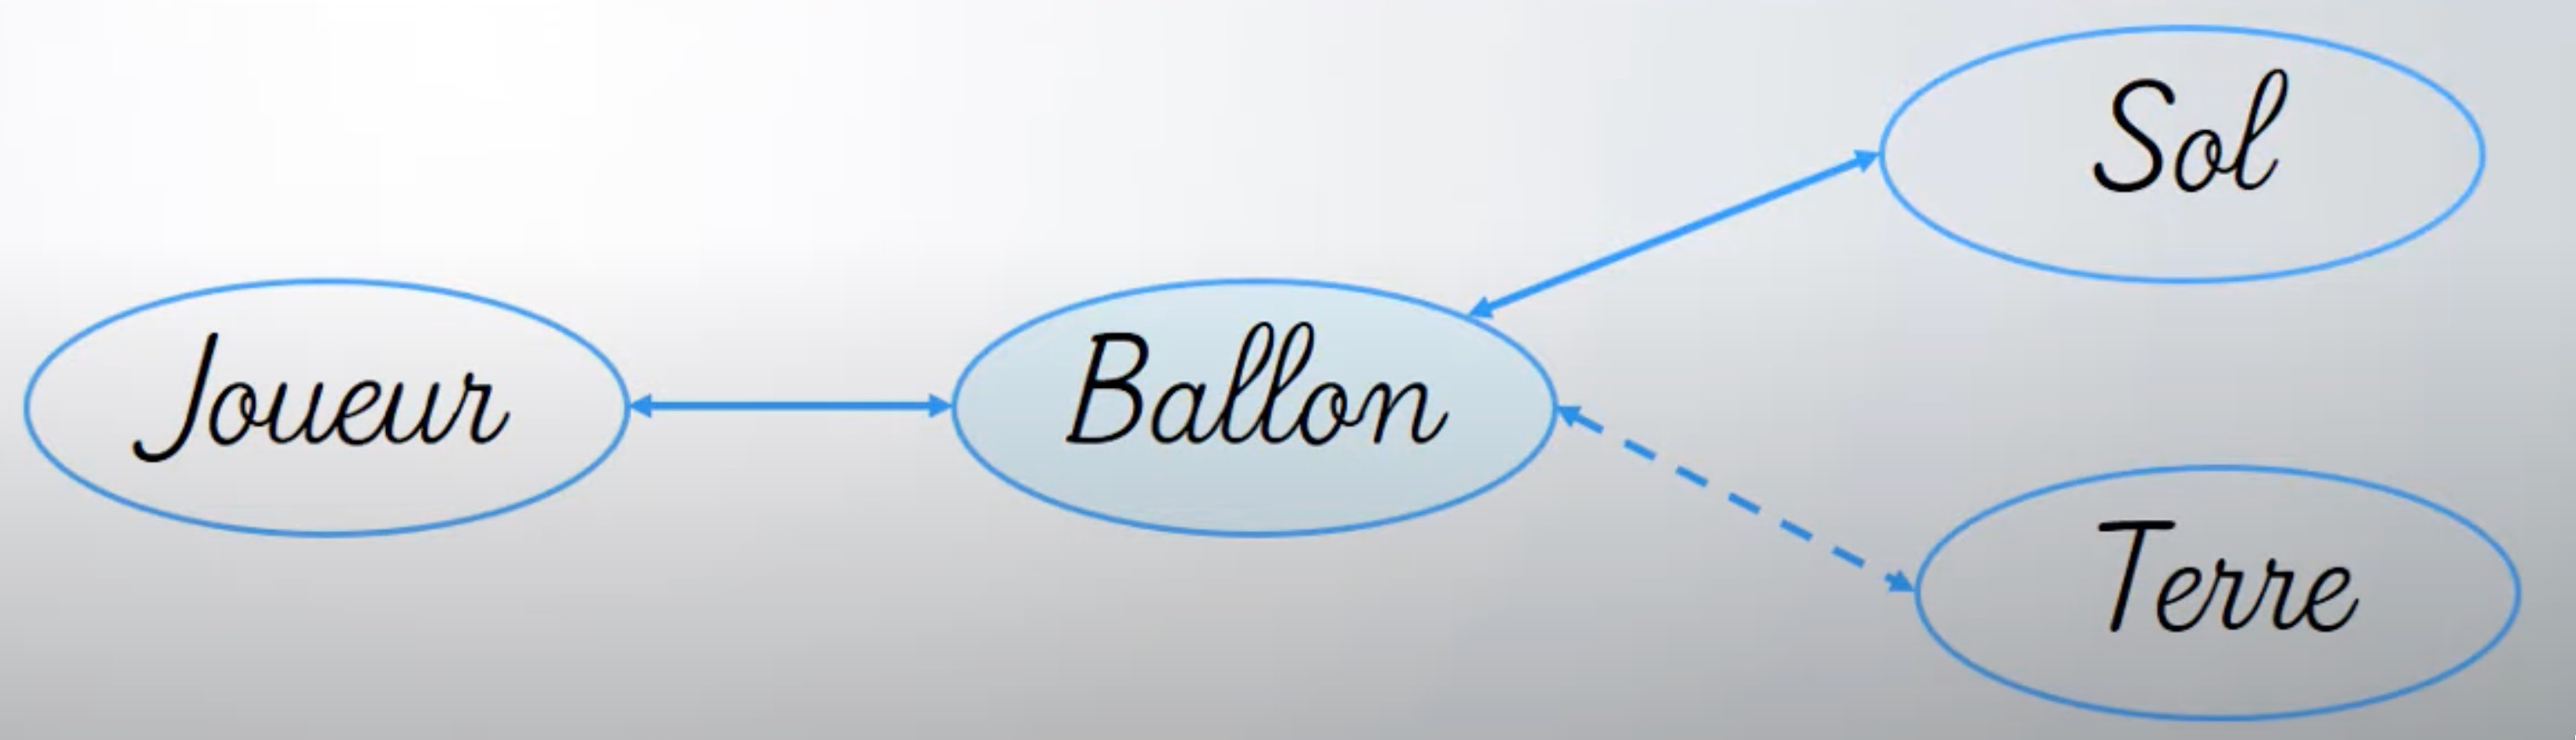
\includegraphics[width=0.8\linewidth]{img/interro_03_corr_01.jpg}
    \end{figure}
    https://www.youtube.com/watch?v=YJ3ocSHImLk
  \end{solution}

  \question[3] Une bille en métal roule sur le sol. Un aimant est placé à 50 cms de la bille et attire la bille vers lui. Réaliser le diagramme objet-intéraction de la bille sur le sol.
  \begin{solution}

    La bille est soumise :
\begin{compactitem}
    \item à la force de contact avec le sol ;
    \item aux forces de frottements de l'air (négligeables ici) ;
    \item à la force d'attraction (action à distance) de la Terre ;
    \item à la force d'attraction (action à distance) de l'aimant.
\end{compactitem}

Le diagramme objet-interaction est alors le suivant (les frottements ne sont pas représentés ici) :

    \begin{figure}[H]
      \centering
      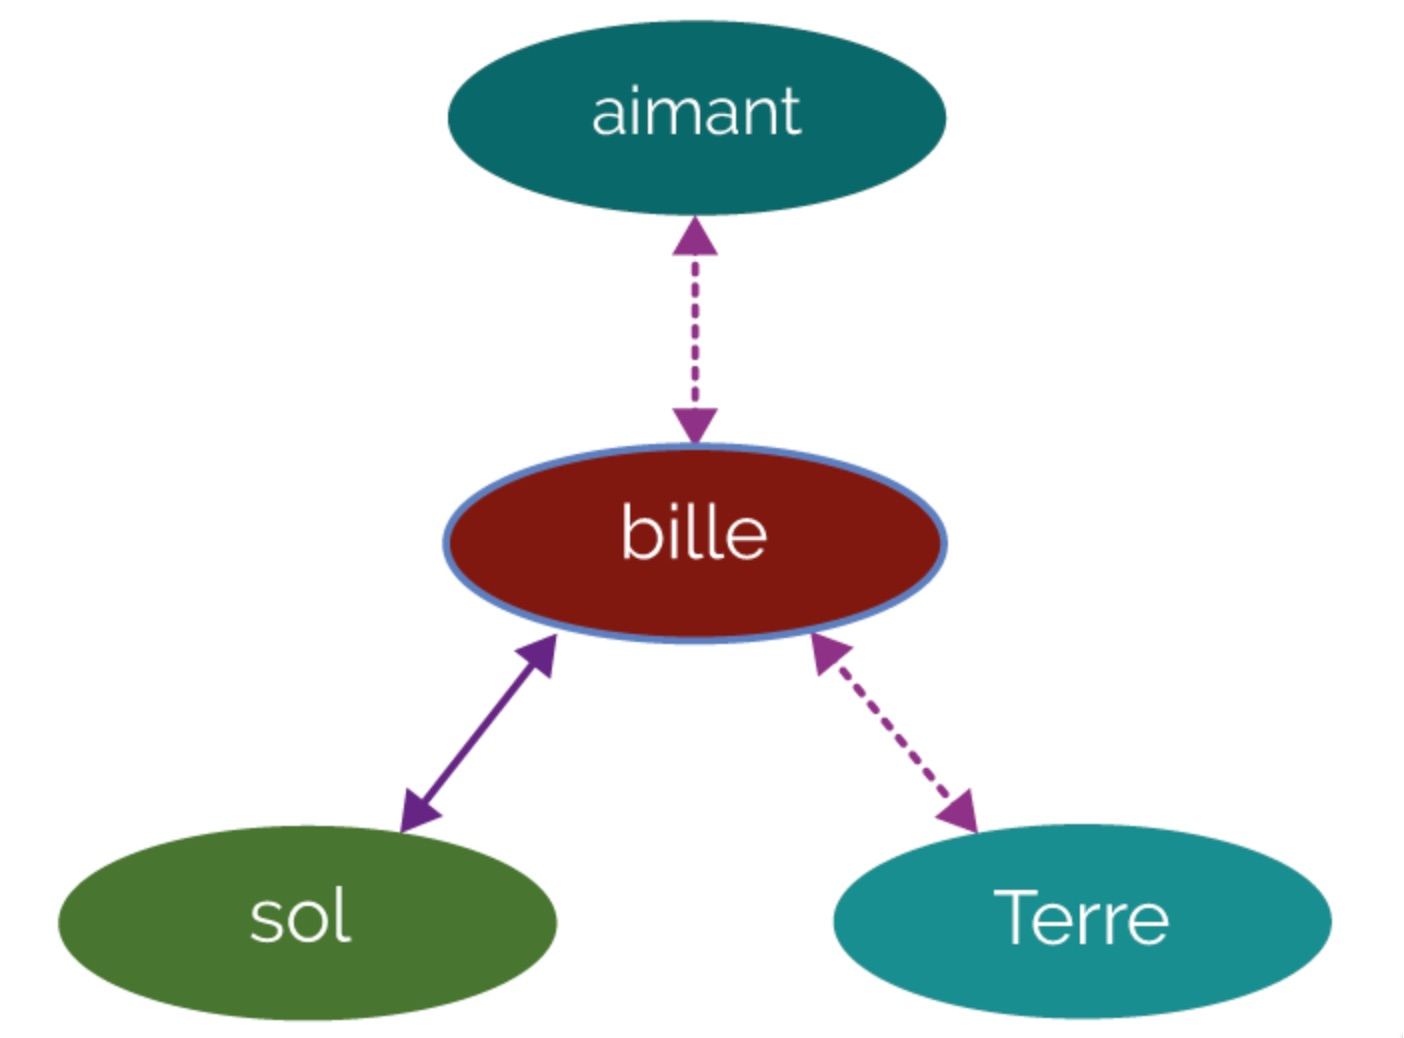
\includegraphics[width=0.7\linewidth]{img/interro_03_corr_02.jpg}
    \end{figure}
    https://www.maxicours.com/se/cours/les-diagrammes-objet-interaction/
  \end{solution}
\end{questions}

\section*{Exercice 3 : Forces (2 points)}
\begin{questions}
  \question[2] Représenter la force exercée par le marteau sur le clou. On considérera que sa valeur est de $30 N$, et on utilisera l'échelle suivante : $1cm = 10N$.
  \begin{figure}[H]
    \centering
    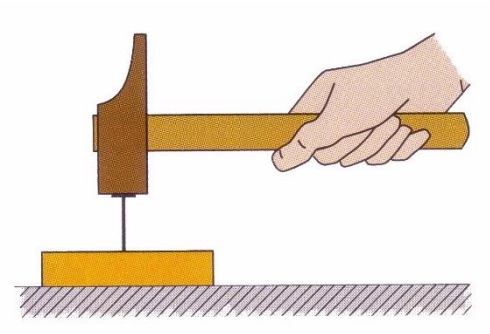
\includegraphics[width=0.7\linewidth]{img/interro_03_01.jpg}
  \end{figure}
\end{questions}

\section*{Exercice 4 - Étude des forces appliquées à une pierre de curling (8 points)}

Le curling est un sport olympique qui consiste à lancer en ligne droite une pierre de 20 kg sur la glace et de la diriger vers une cible appelée maison. La glace est balayée par deux joueurs afin de guider la pierre jusqu’à la cible.
\begin{figure}[H]
  \centering
  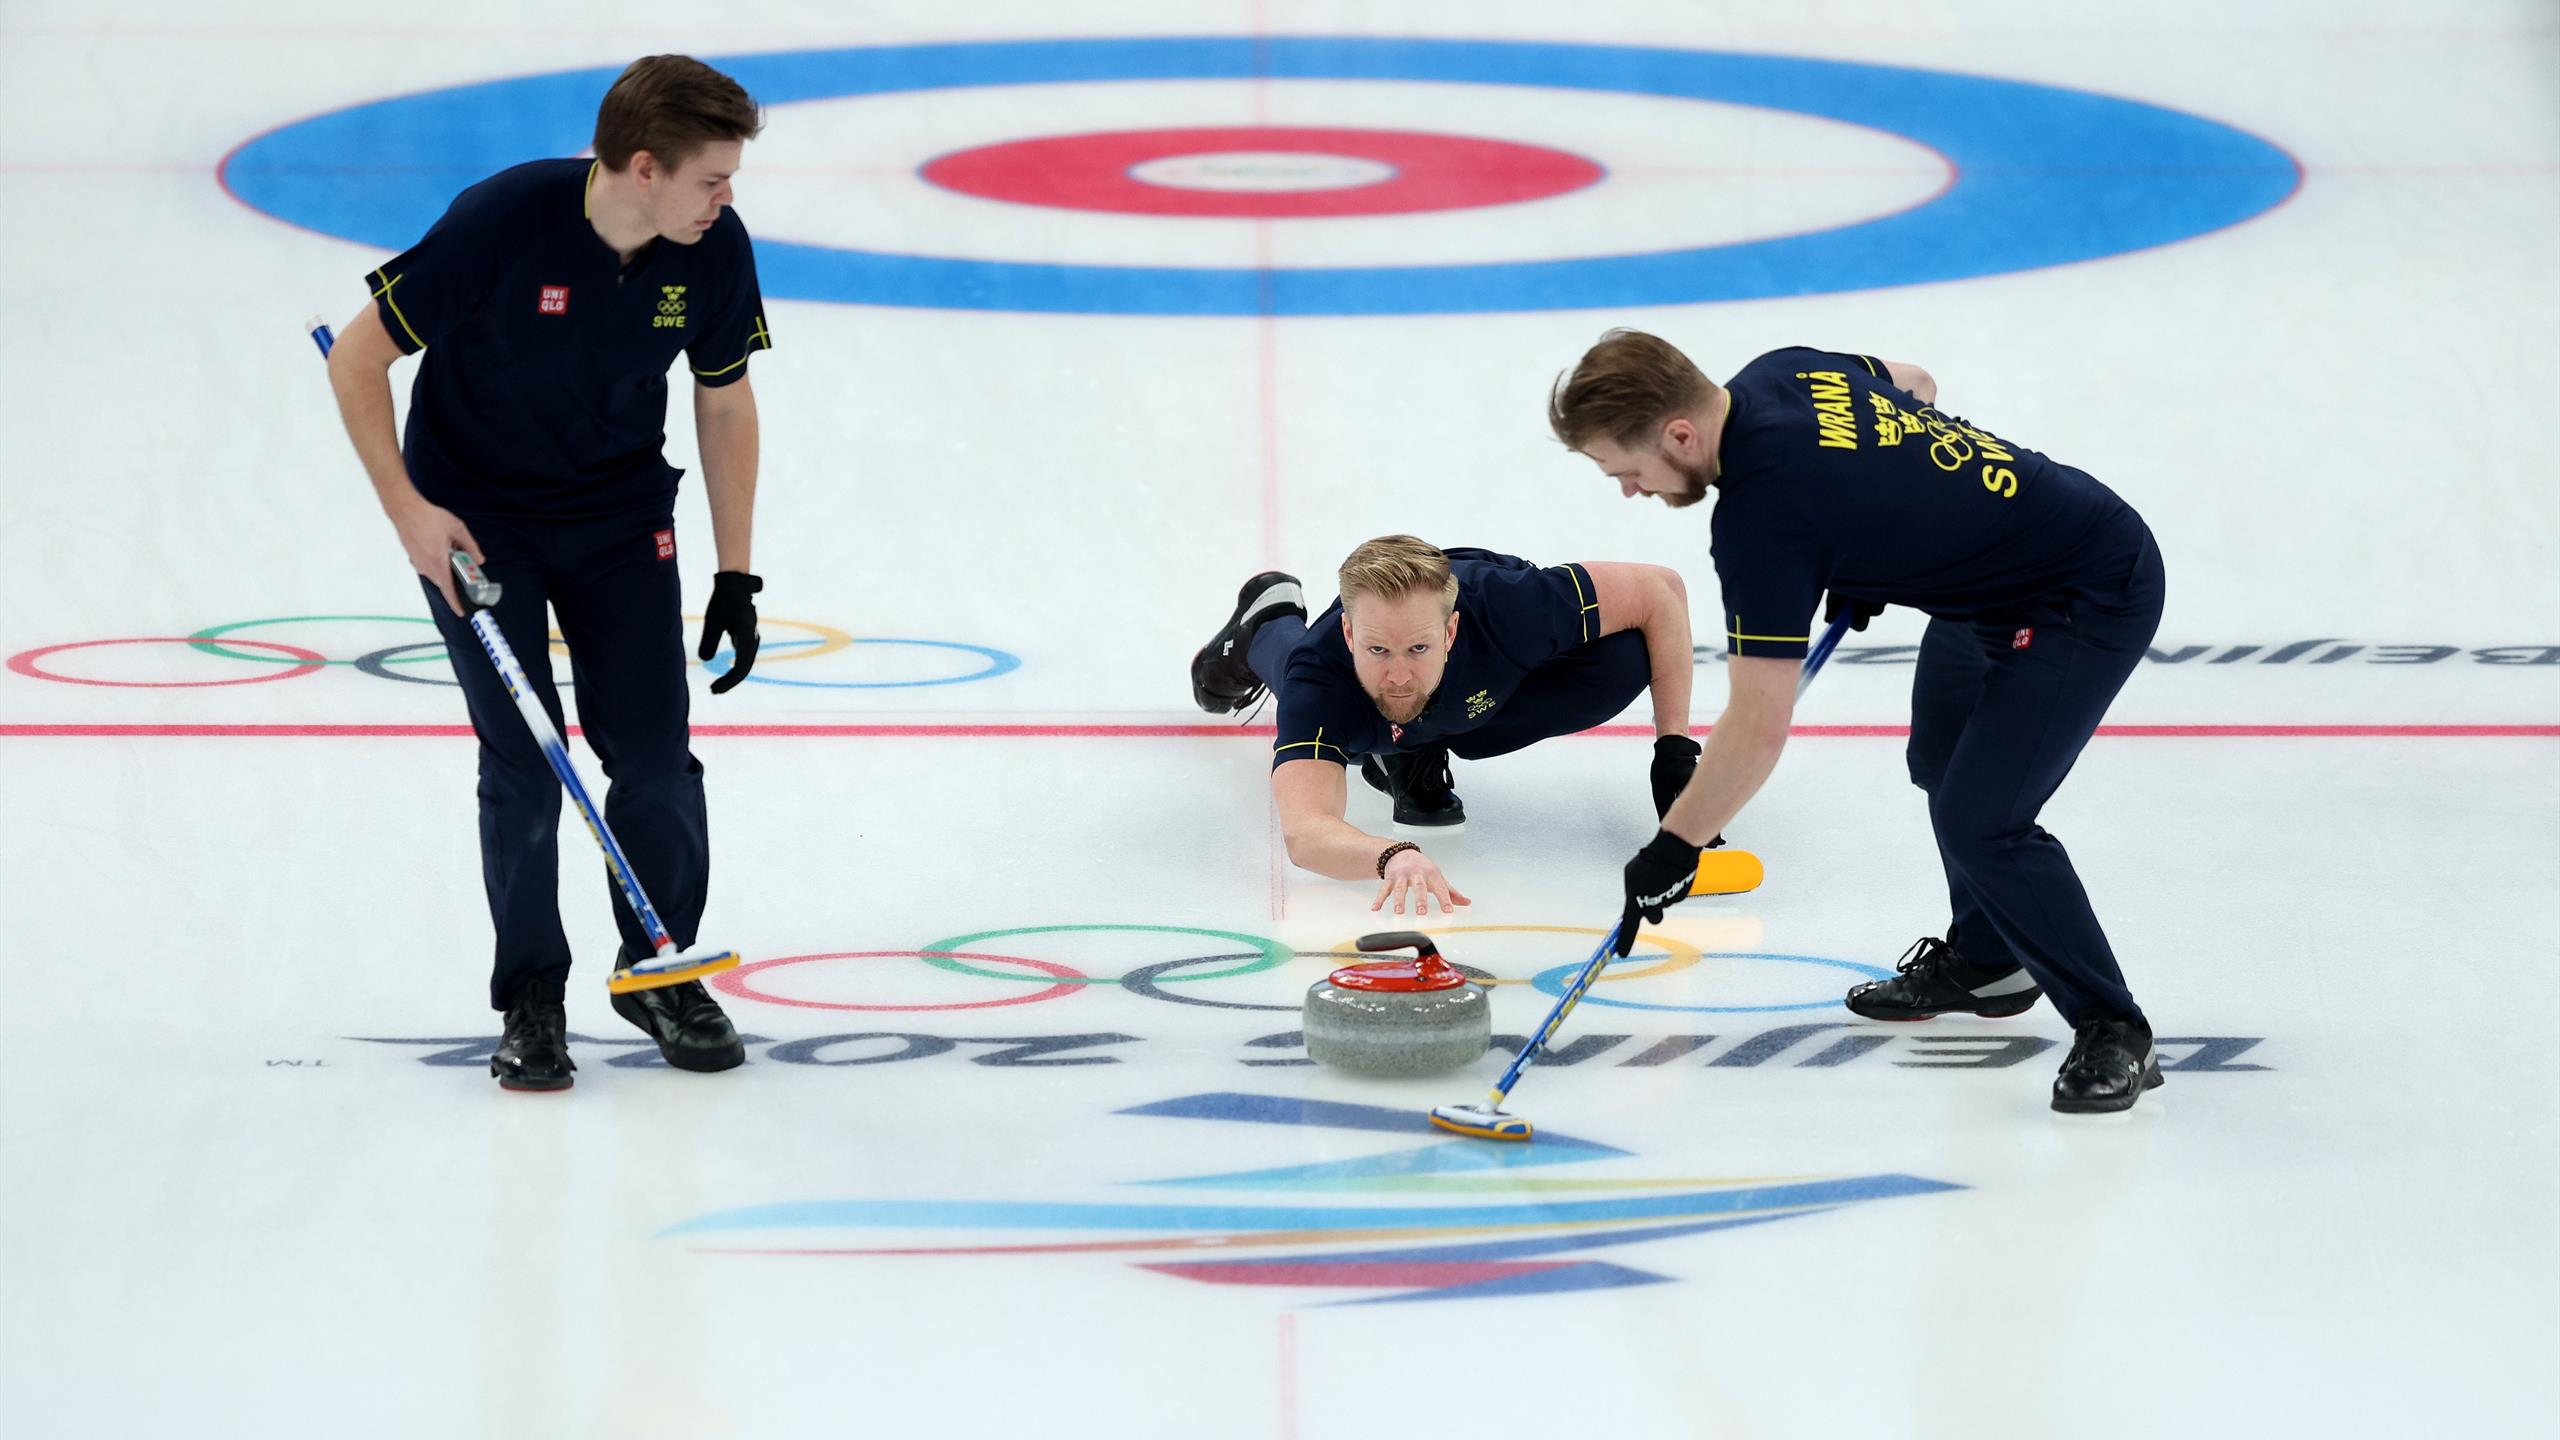
\includegraphics[width=0.6\linewidth]{img/interro_03_02.jpg}
\end{figure}
\begin{questions}
  \question[2] Faire le bilan des interactions qui s’exercent sur la pierre lors de son mouvement, en tenant compte des frottements de la pierre sur la glace.
  \begin{solution}
    Une pierre de curling en mouvement est soumise aux forces suivantes :
    
    \begin{itemize}
        \item \textbf{La force de frottement} $\vec{f_1}$ :  
        \begin{compactitem}
            \item \textbf{Direction} : horizontale, parallèle à la surface de la glace.
            \item \textbf{Sens} : opposé au mouvement de la pierre.
            \item \textbf{Norme} : dépend de la rugosité de la glace et de la masse de la pierre.
            \item \textbf{Point d'application} : on peut considérer qu’elle s’applique au centre de la surface de contact entre la pierre et la glace.
        \end{compactitem}
        
        \item \textbf{Le poids} $\vec{P}$ :  
        \begin{compactitem}
            \item \textbf{Direction} : verticale.
            \item \textbf{Sens} : vers le bas (vers le centre de la Terre).
            \item \textbf{Norme} : $P = mg$, où $m$ est la masse de la pierre et $g$ l’accélération gravitationnelle ($g \approx 9.81~\text{m/s}^2$).
            \item \textbf{Point d'application} : au centre de gravité de la pierre.
        \end{compactitem}
    
        \item \textbf{La réaction du sol} $\vec{R}$ :  
        \begin{compactitem}
            \item \textbf{Direction} : verticale, perpendiculaire à la glace.
            \item \textbf{Sens} : vers le haut, opposé au poids.
            \item \textbf{Norme} : $R = P$ (si la pierre est en équilibre vertical, c’est-à-dire sans enfoncement dans la glace).
            \item \textbf{Point d'application} : au centre de la surface de contact entre la pierre et la glace.
        \end{compactitem}
    \end{itemize}
    
    Ainsi, $\vec{P}$ et $\vec{R}$ se compensent verticalement, tandis que $\vec{f_1}$ agit pour ralentir la pierre horizontalement.
    \end{solution}
  \question[2] Modéliser les interactions par des forces en les représentant à l’aide d’un schéma.
  \question[2] En l’absence de frottements, quel serait le mouvement de la pierre de curling une fois lâchée par le lanceur ? Justifier votre réponse en utilisant un principe fondamental de la mécanique.
  \question[2] En déduire le rôle des deux joueurs qui balaient devant la pierre au cours de son mouvement.
\end{questions}



\end{document}
